\section{Flow correlations}
\label{sec:ps:flow}
%5. Flow Correlations & Flow & PID Flow (PS)
%- Geometric fluctuations and origin of v_n vs ecc_n (Glauber, v3)
%- non-PID flow (ALICE first results)
%- PID flow (ALICE v2 scaling)
%- 2PC (CMS v_n?)
%- Event plane (ATLAS EP)
%- Explaining the ridge (2PC from 3 experiments)
%- Flow fluctuations
%- Event plane correlations
%- Success of viscous hydro
%- Comparison with RHIC
%- Flow in p+Pb (ridge, double ridge, PID)
%- Open questions

\begin{figure}[!htb]
\begin{center}
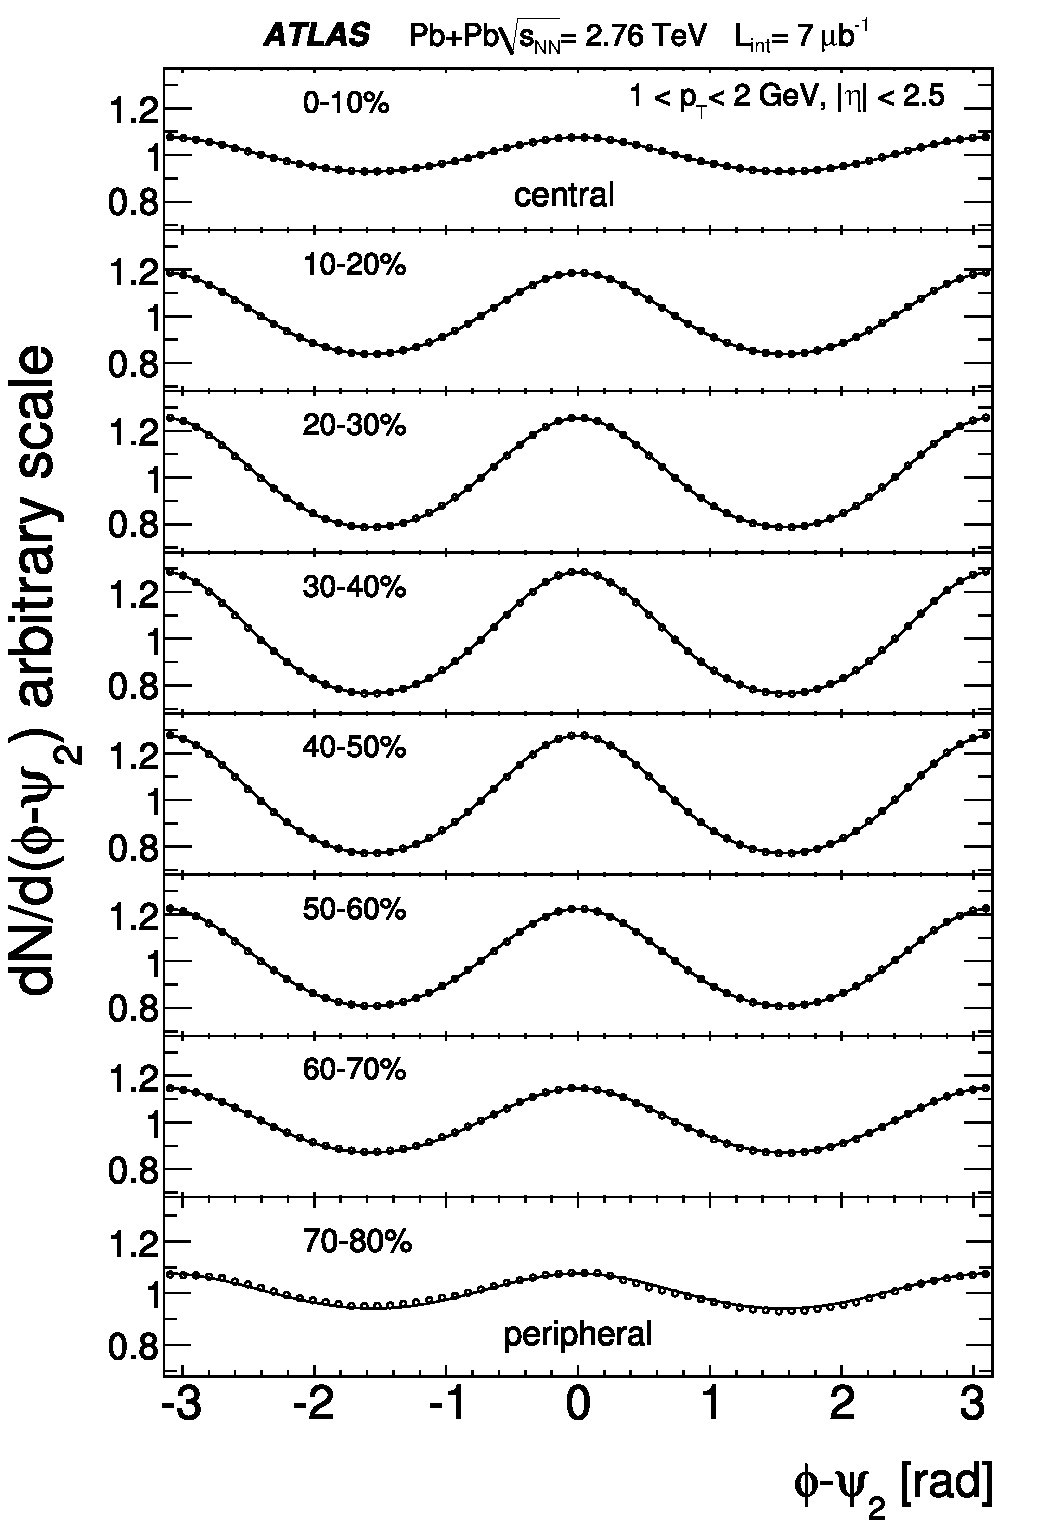
\includegraphics[width=0.49\textwidth]{flowcorrelations_figs/atlas_v2_fig_02.pdf}
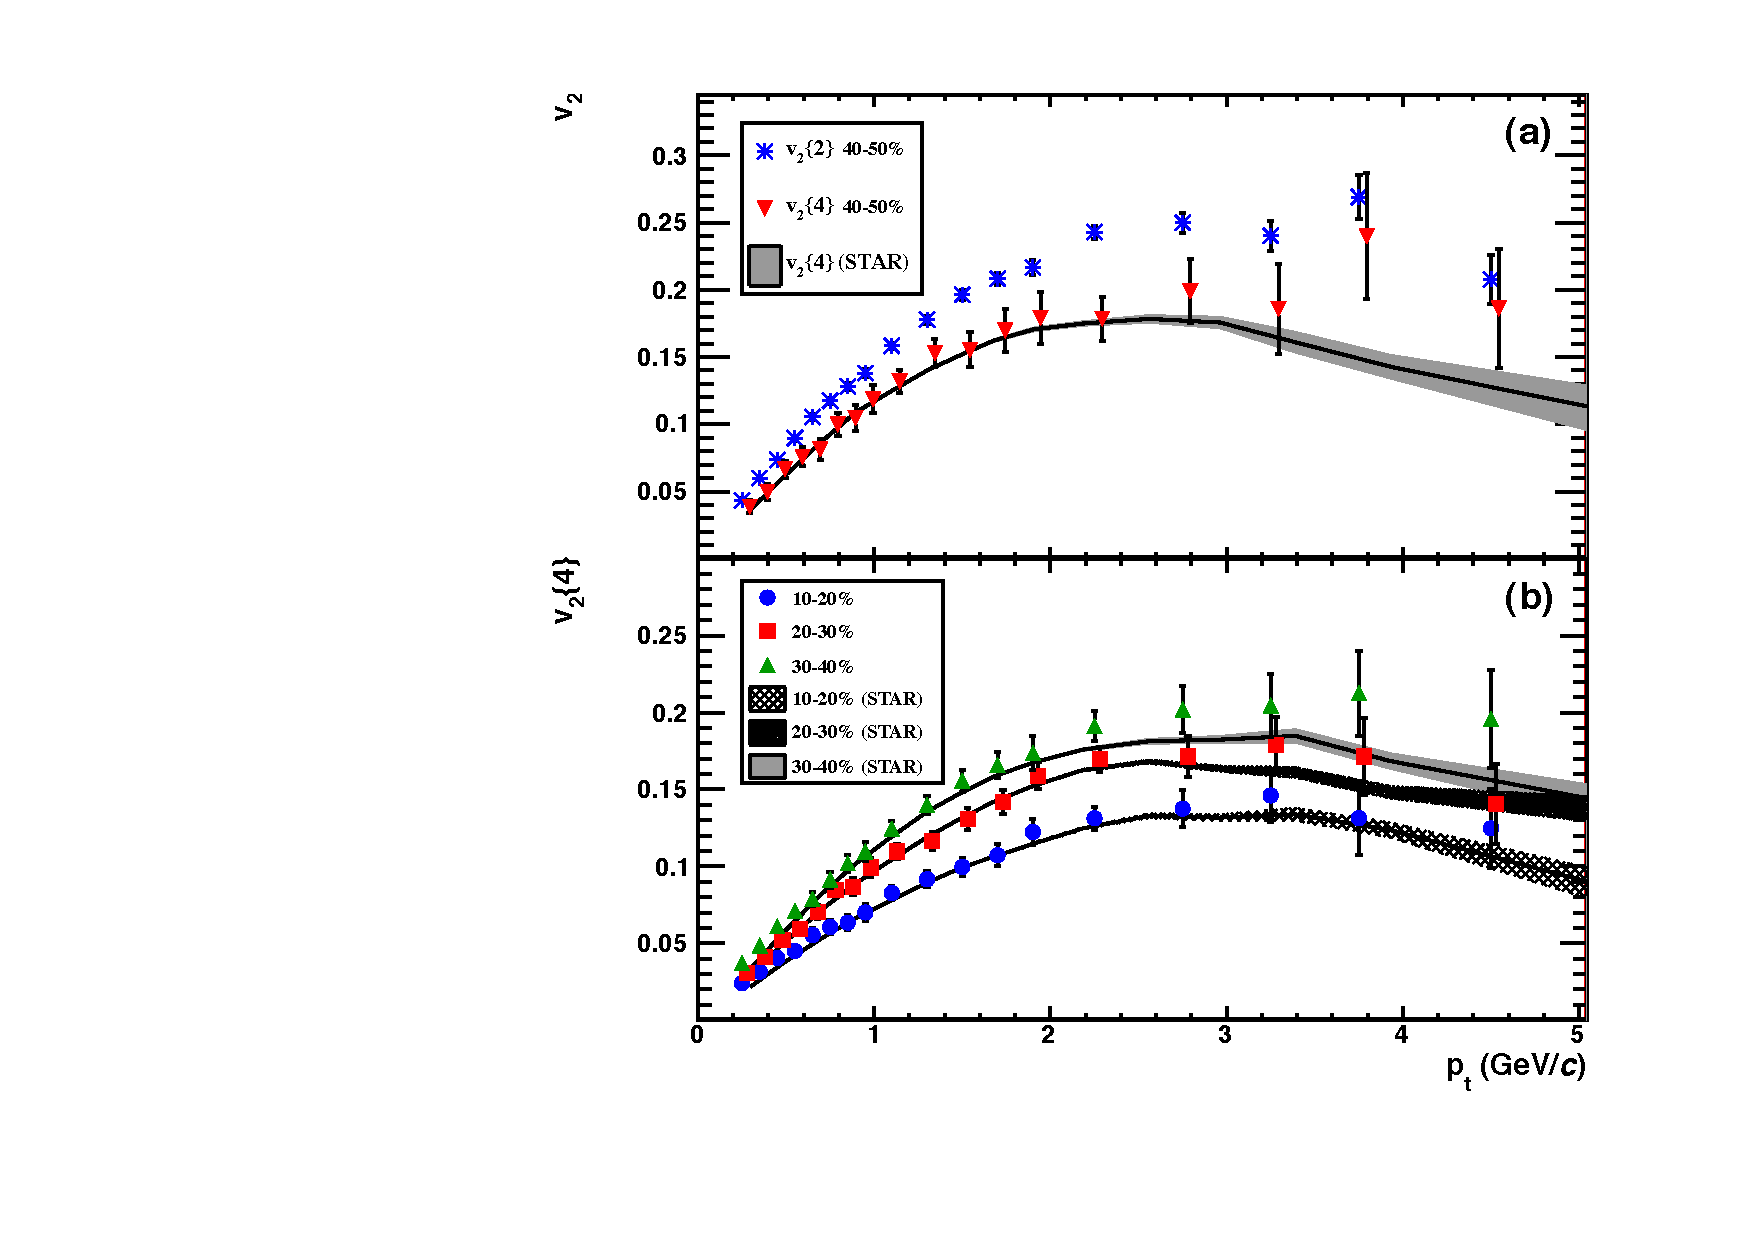
\includegraphics[width=0.49\textwidth]{flowcorrelations_figs/fig2.pdf}
\caption[]{(left) ATLAS data showing the evolution of anisotropy relative to the reaction plane, as a function of centrality (right) First ALICE data on \vtwo in Pb+Pb collisions at the LHC.}
\label{fig:pas:fc:firstreusults}
\end{center}
\end{figure}

\begin{figure}[!htb]
\begin{center}
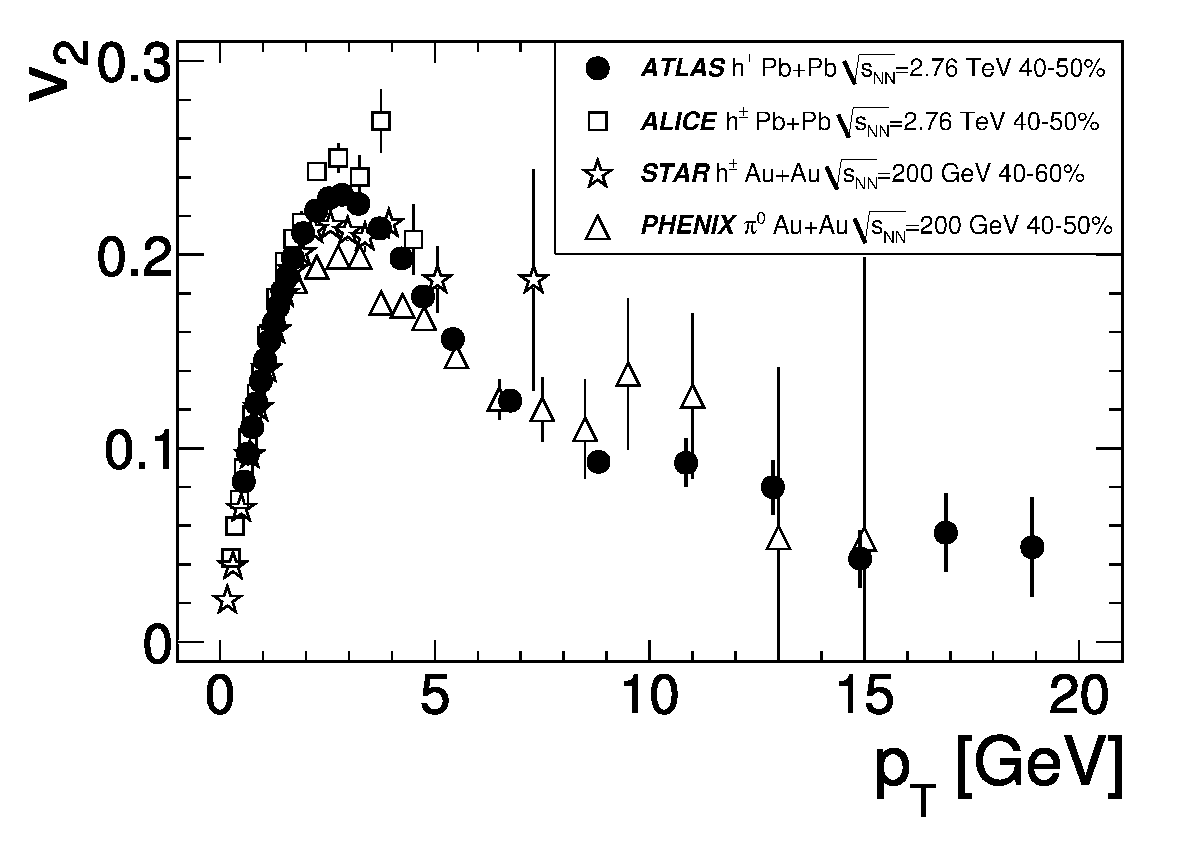
\includegraphics[width=0.49\textwidth]{flowcorrelations_figs/atlas_v2_fig_06.pdf}
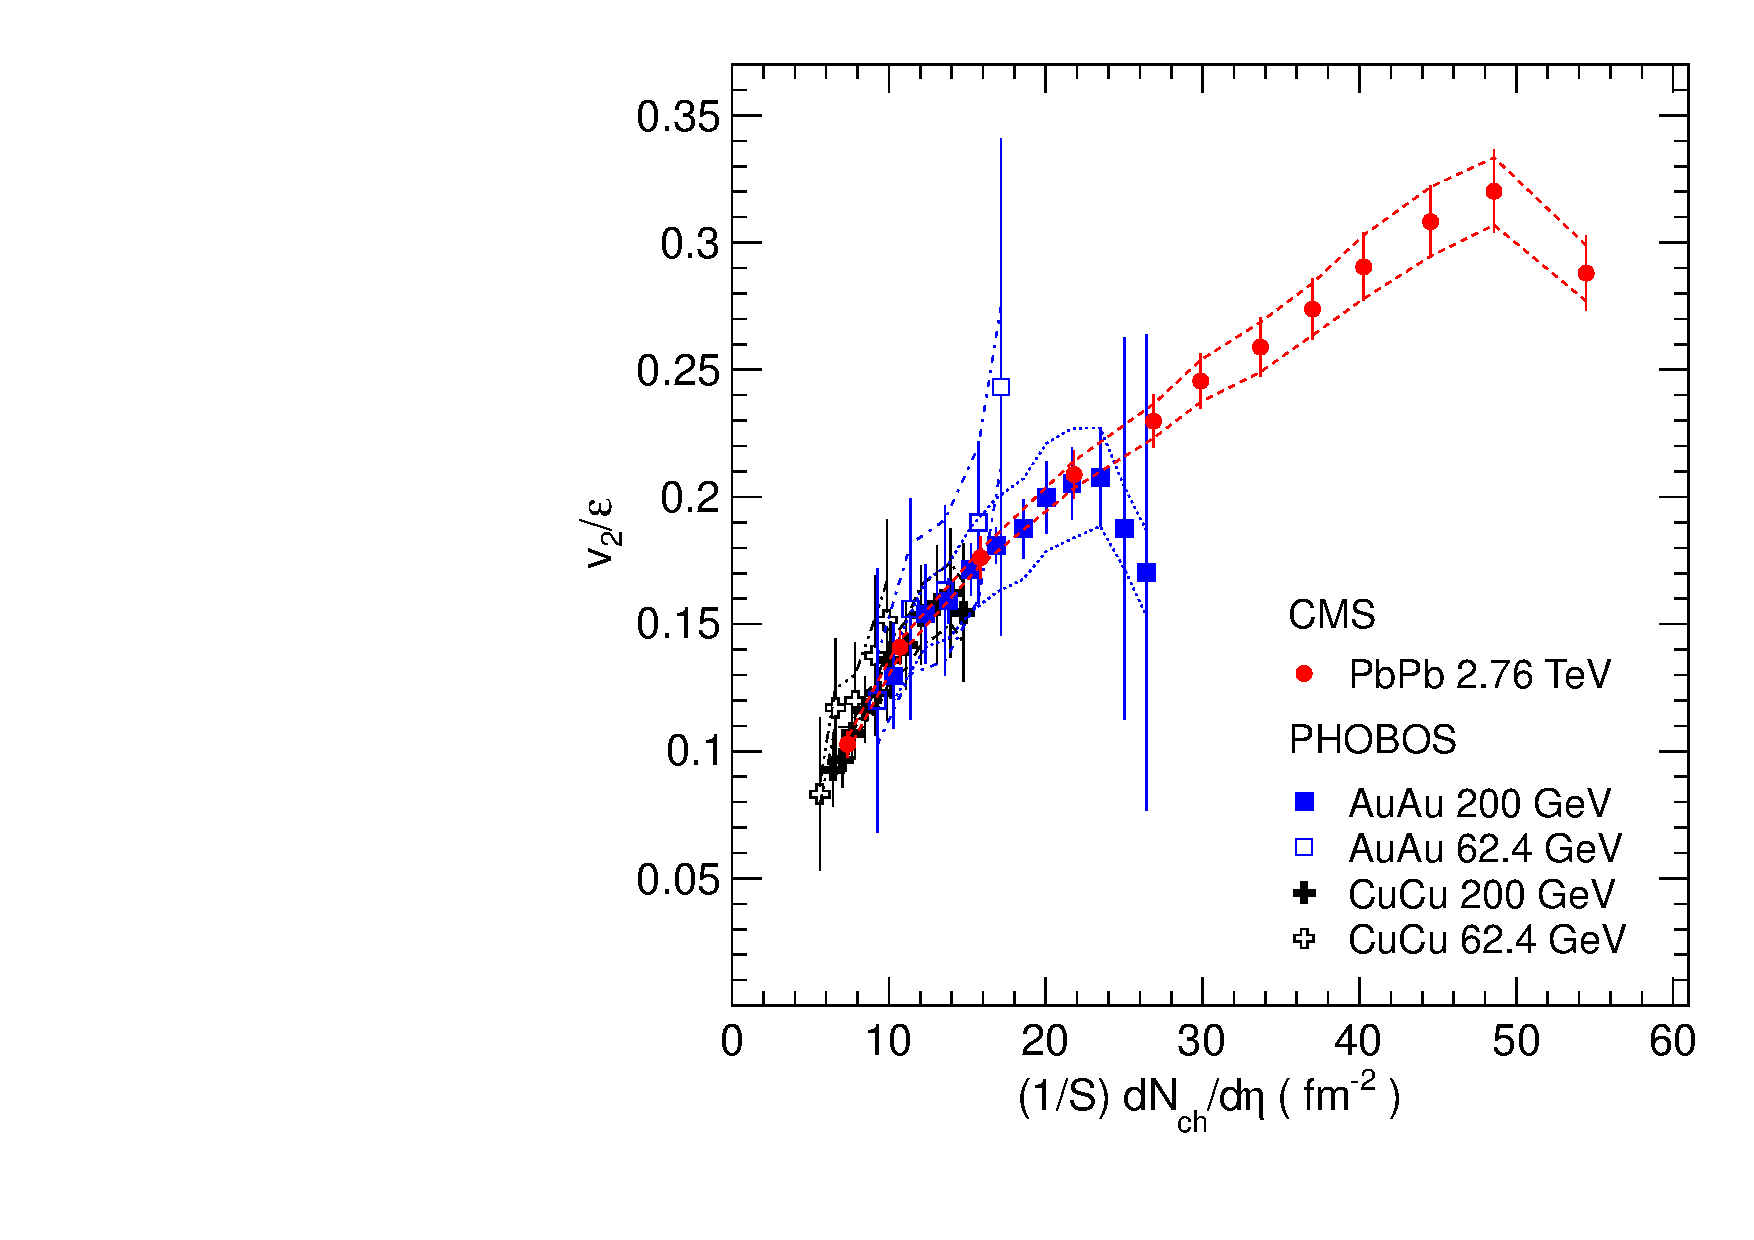
\includegraphics[width=0.49\textwidth]{flowcorrelations_figs/v2eps_dNdetaoverS_PHOBOS.pdf}
\caption[]{(left) ATLAS data showing the invariance of $\vtwo( \pT )$ with beam energy (right) CMS compilation showing the observed scaling of $\vtwo /\epsilon$ vs. $(1/S) dN_{ch}/d\eta$.}
\label{fig:pas:scaling}
\end{center}
\end{figure}

\begin{figure}[!htb]
\begin{center}
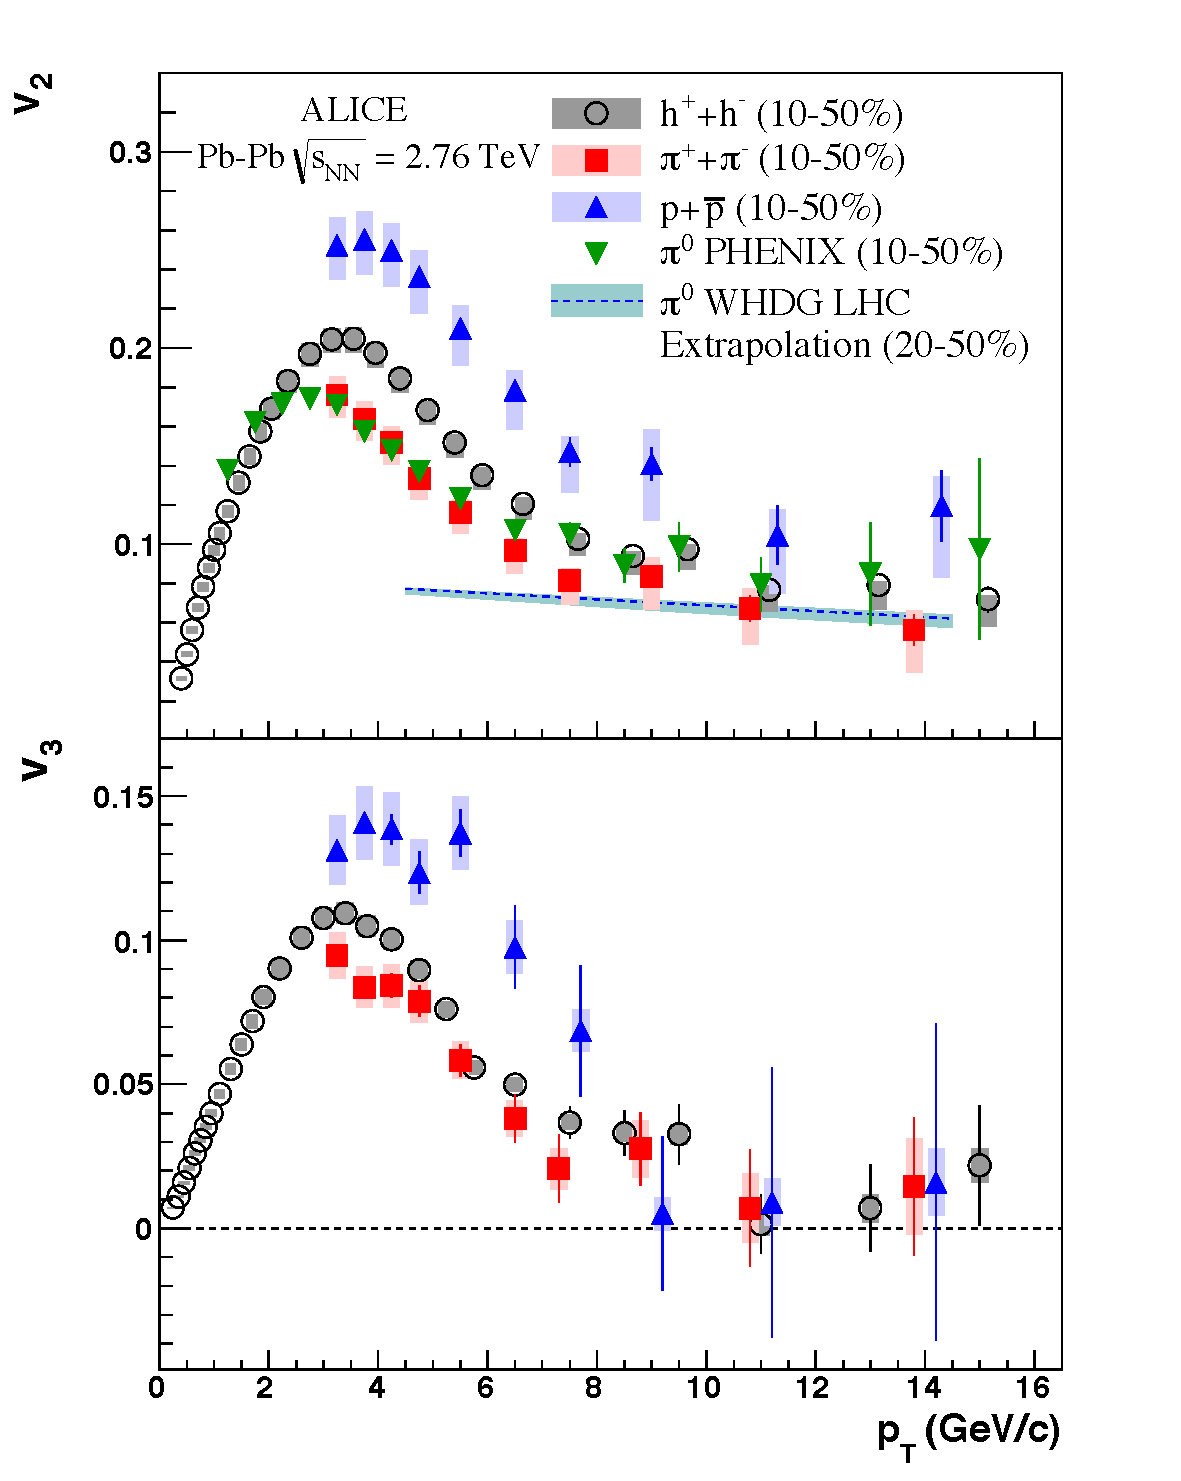
\includegraphics[width=0.49\textwidth]{flowcorrelations_figs/fig5_vn_pid.pdf}
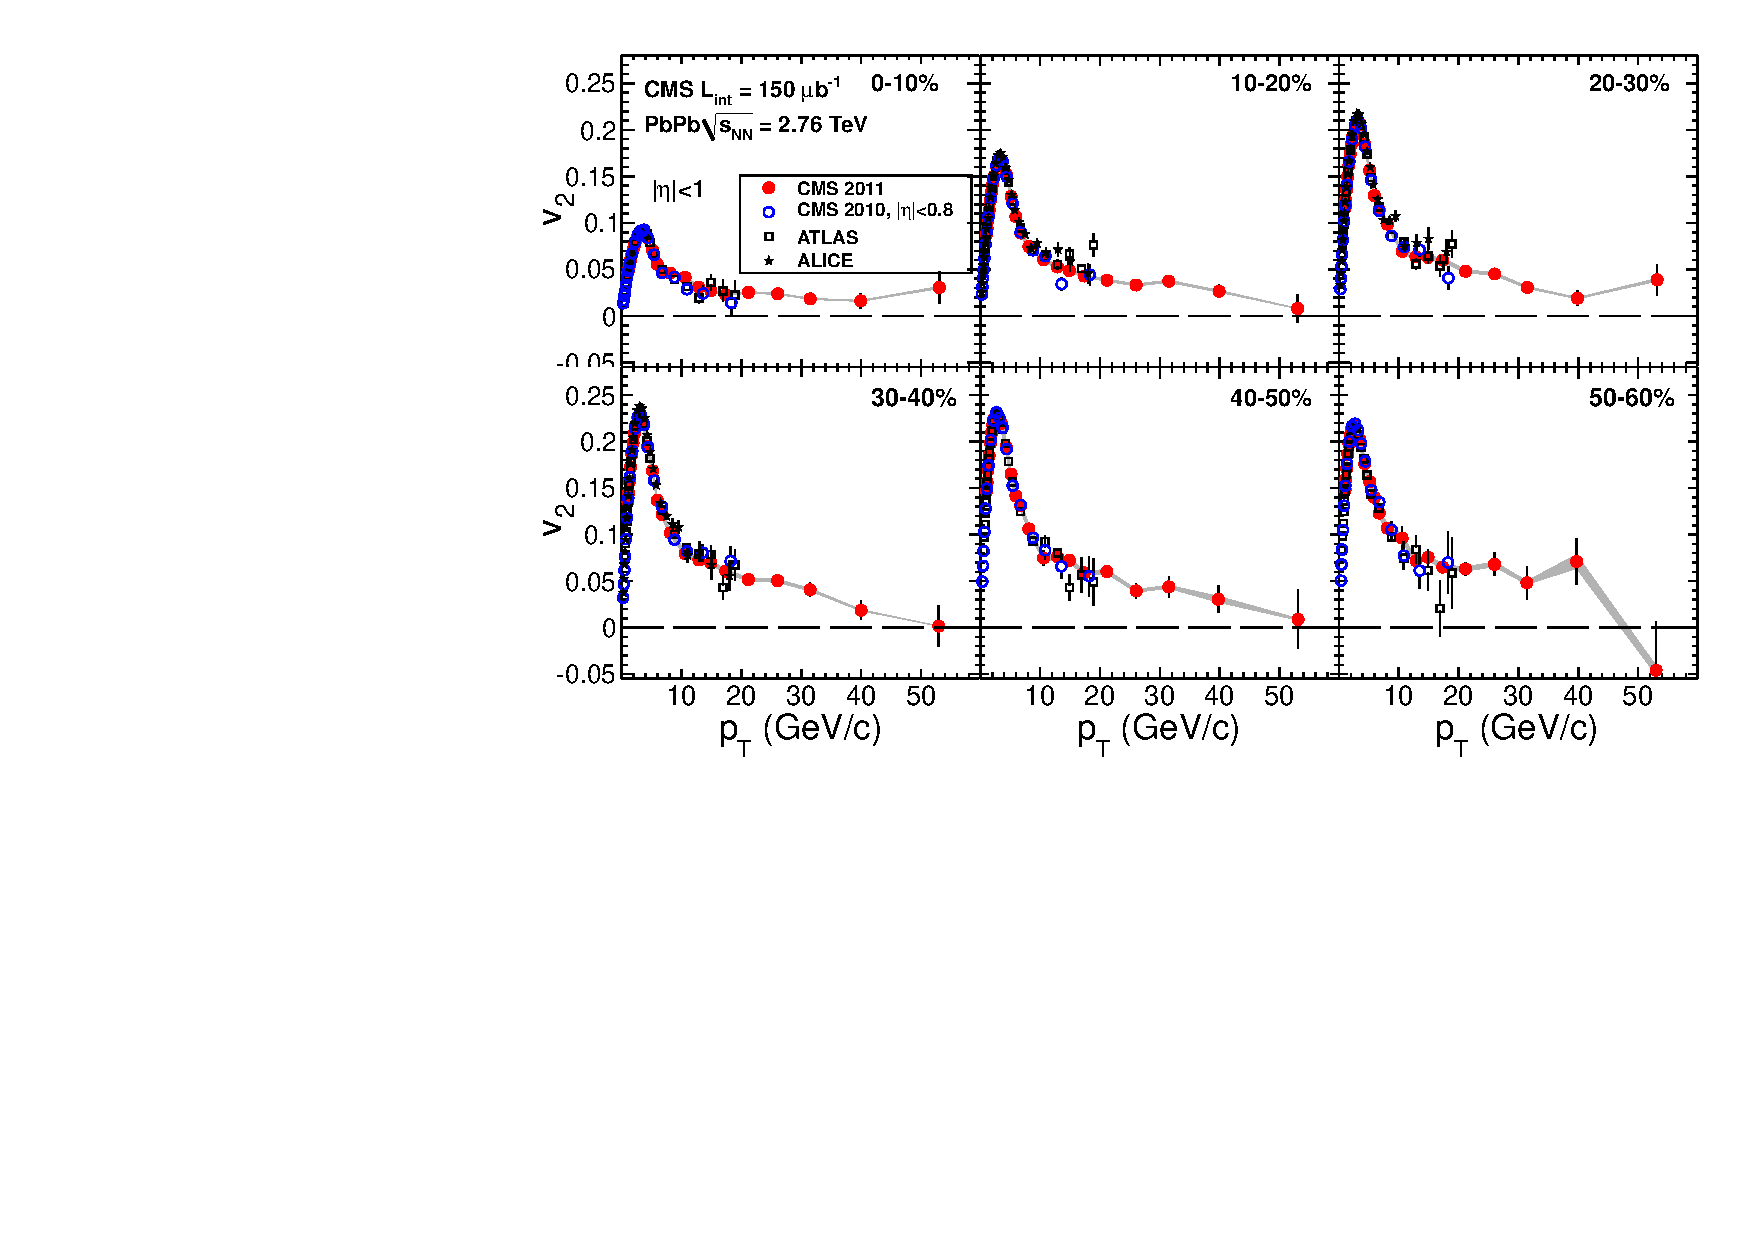
\includegraphics[width=0.49\textwidth]{flowcorrelations_figs/v2_pt_ep_atlas_alice_eta0-1_band_v5.pdf}
\caption[]{(left) ALICE data showing $\vtwo(\pT)$ for identified hadrons, for $|\eta|<0.8$ (right) CMS data showing the $\vtwo$ for unidentified hadrons at very high \pT, out to 50 GeV}
\label{fig:pas:fc:highpt}
\end{center}
\end{figure}

\begin{figure}[!htb]
\begin{center}
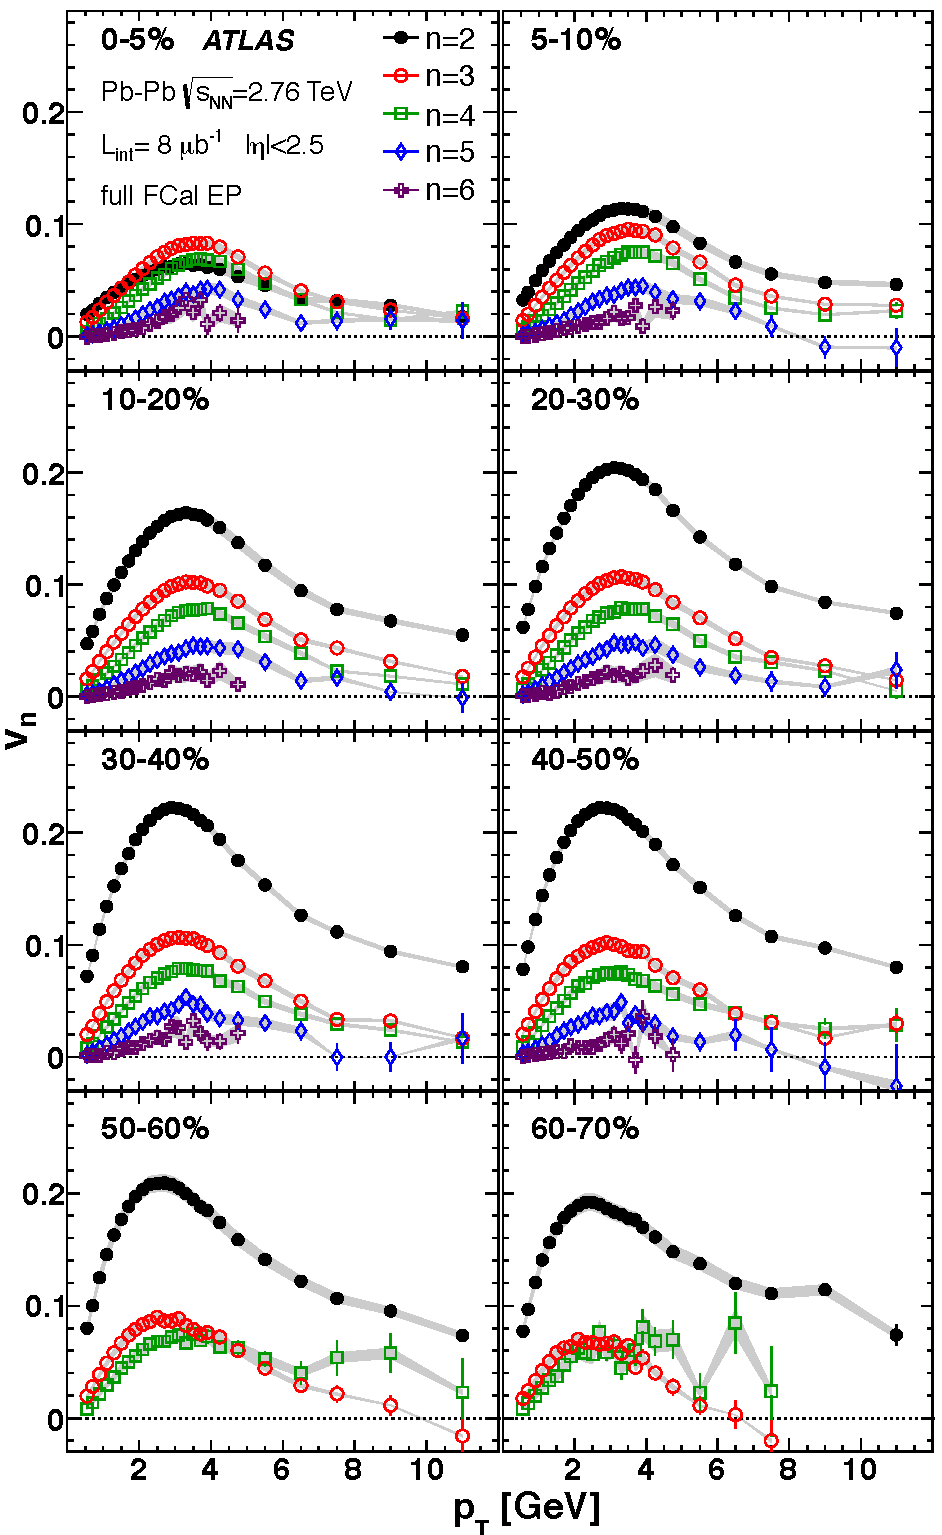
\includegraphics[width=0.49\textwidth]{flowcorrelations_figs/atlas_vn_fig_04.pdf}
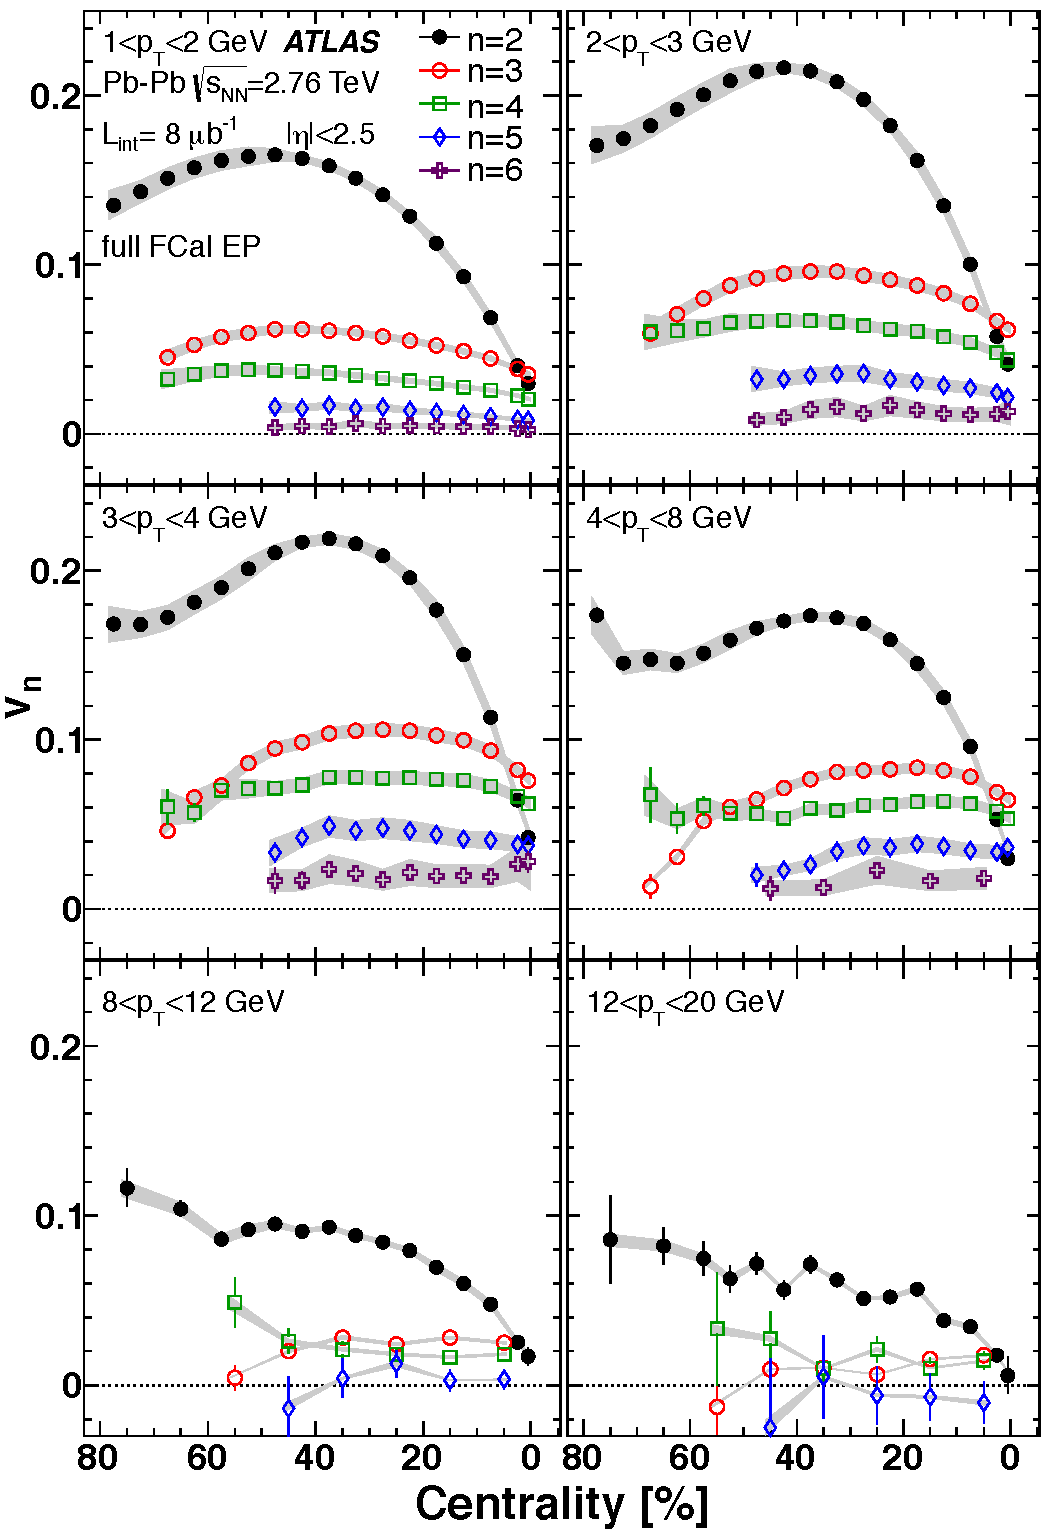
\includegraphics[width=0.49\textwidth]{flowcorrelations_figs/atlas_vn_fig_05.pdf}
\caption[]{(left) ATLAS data showing $v_n(\pT)$ for different centrality intervals and $|\eta|<2.5$, for $n=2-6$.  Very little dependence on $\eta$ is observed.  
(right) The same ATLAS data, in \pT intervals, showing the centrality dependence of $v_n$.}
\label{fig:pas:fc:vn}
\end{center}
\end{figure}

\begin{figure}[!htb]
\begin{center}
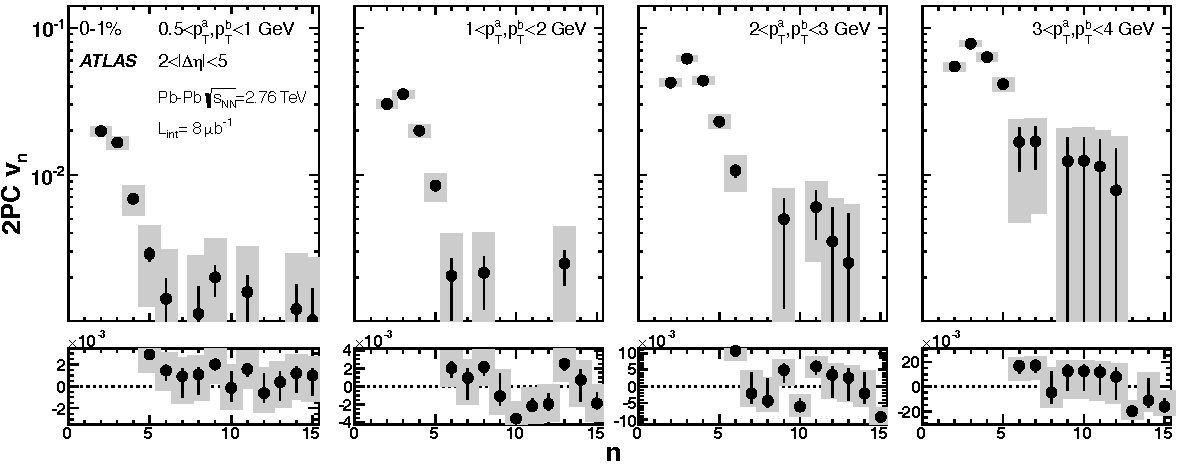
\includegraphics[width=0.98\textwidth]{flowcorrelations_figs/atlas_vn_fig_13.pdf}
\caption[]{
ATLAS data showing the $n$ dependence of $v_n$ in four \pT intervals, which are effectively
angular power spectra at different resolution scales.
}
\label{fig:pas:fc:powerspec}
\end{center}
\end{figure}

\begin{figure}[!htb]
\begin{center}
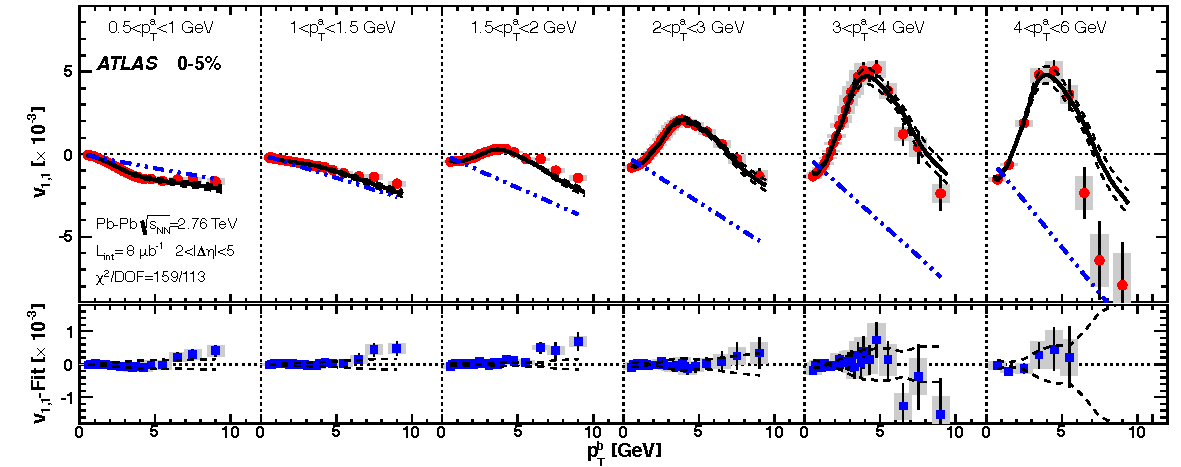
\includegraphics[width=0.98\textwidth]{flowcorrelations_figs/atlas_vn_fig_20a.pdf}
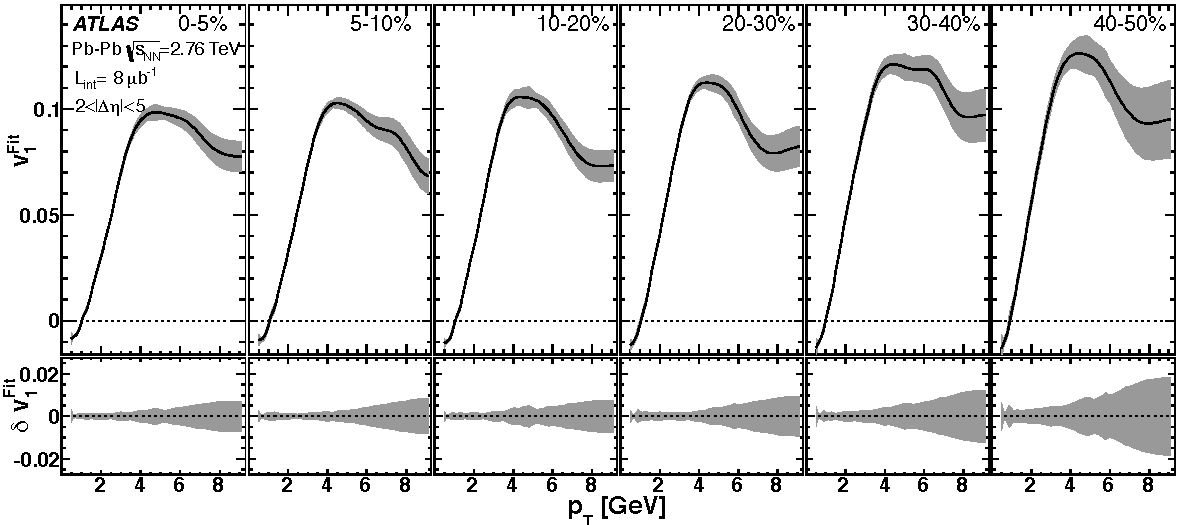
\includegraphics[width=0.98\textwidth]{flowcorrelations_figs/atlas_vn_fig_21.pdf}
\caption[]{
(top) ATLAS data showing the amplitude of $v_{1,1}$ the dipole modulation in the 2-particle correlation function, as a function of $p^b_T$ for ranges in $p^a_T$.  The fit used to extract the functional form of $v_1(\pT)$ is shown.
(bottom) The extracted functional form of $v_1(\pT)$, from the fits shown above, as a function of centrality.
}
\label{fig:pas:fc:v1}
\end{center}
\end{figure}

\begin{figure}[!htb]
\begin{center}
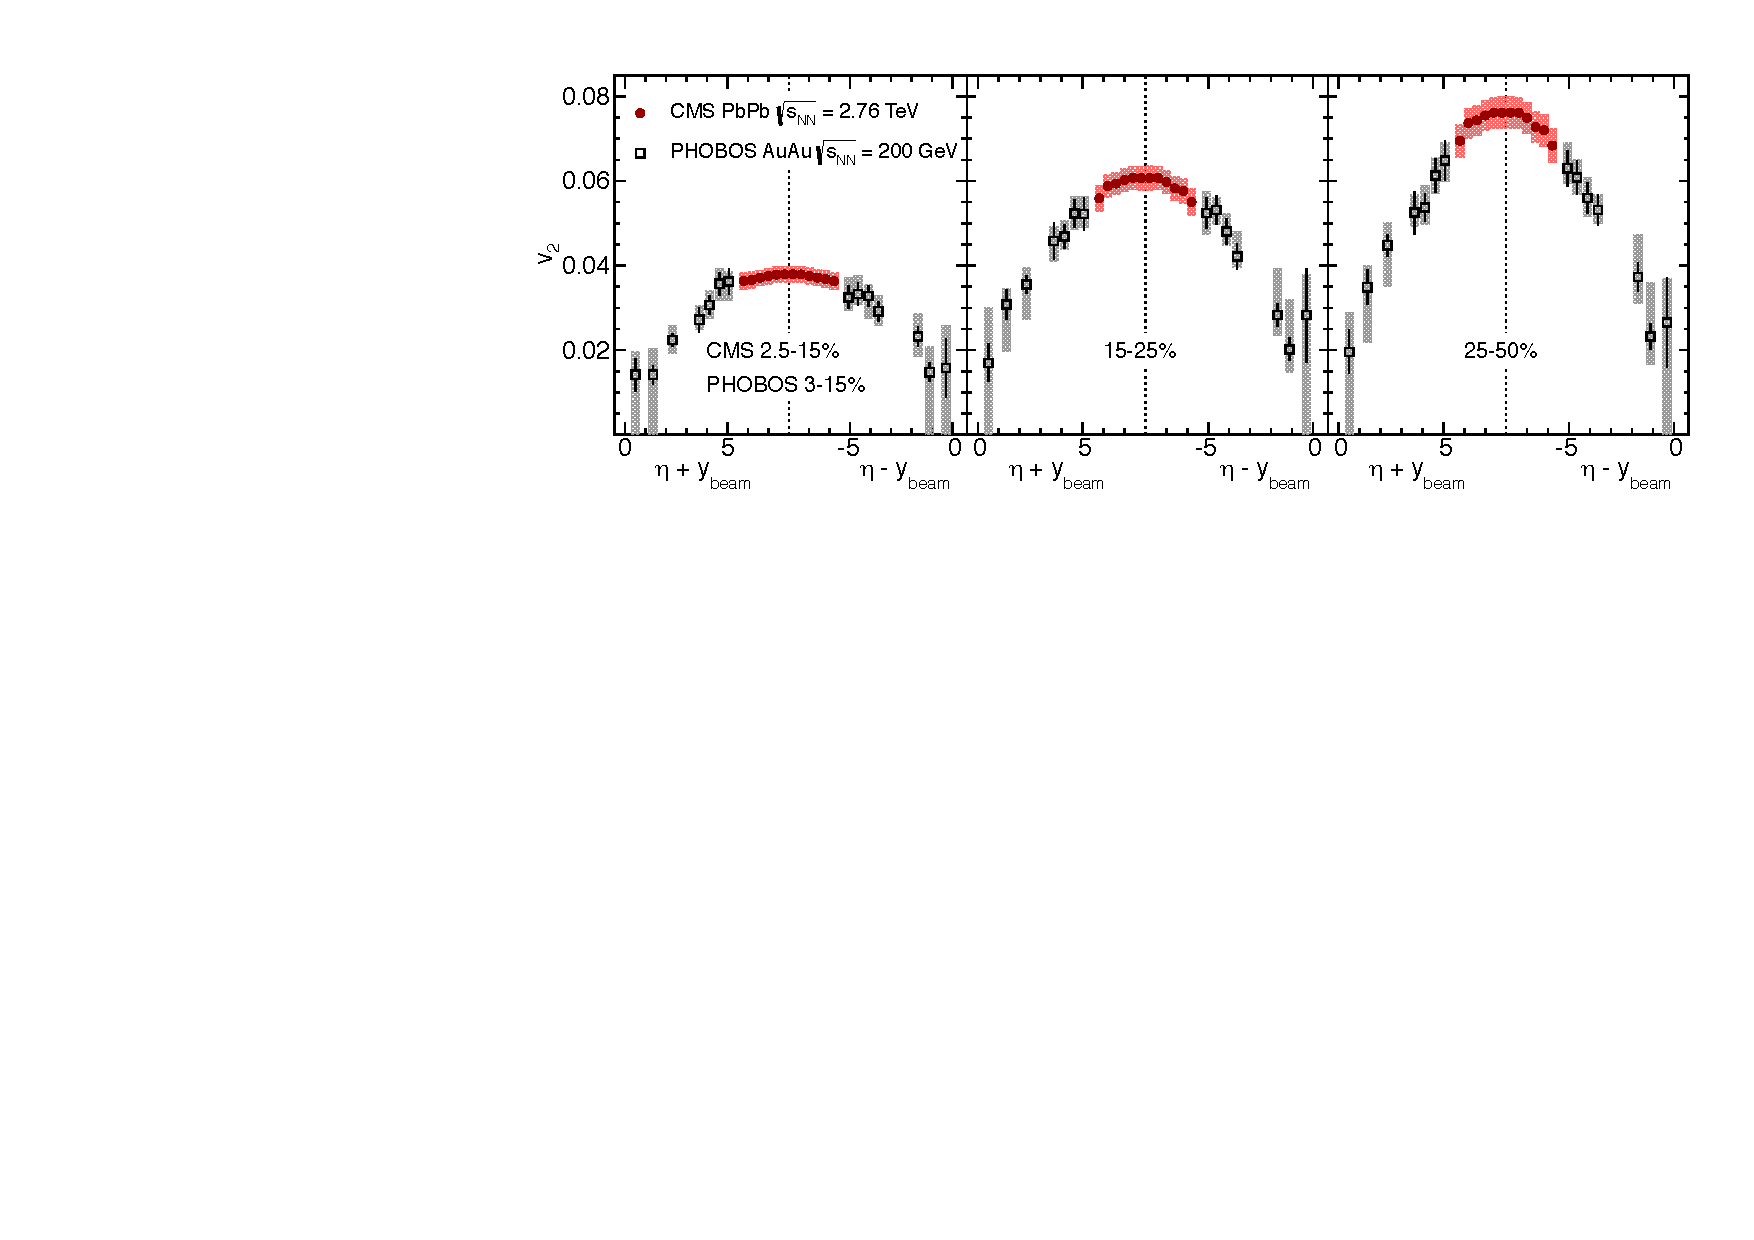
\includegraphics[width=0.98\textwidth]{flowcorrelations_figs/v2_etashifted_3cen_PHOBOS.pdf}
\caption[]{
CMS data showing $\vtwo$ for unidentified hadrons as a function of $\eta - y_{\mathrm{beam}}$, averaged over $0 <\pT < 3$ GeV (using an extrapolation procedure to cover $\pT <300$ Mev).
Results are compared to data from $\sqrt{s_{NN}}=200$ GeV
at large $\eta$ from the PHOBOS experiment at RHIC.
}
\label{fig:pas:fc:limfrag}
\end{center}
\end{figure}

\begin{figure}[!htb]
\begin{center}
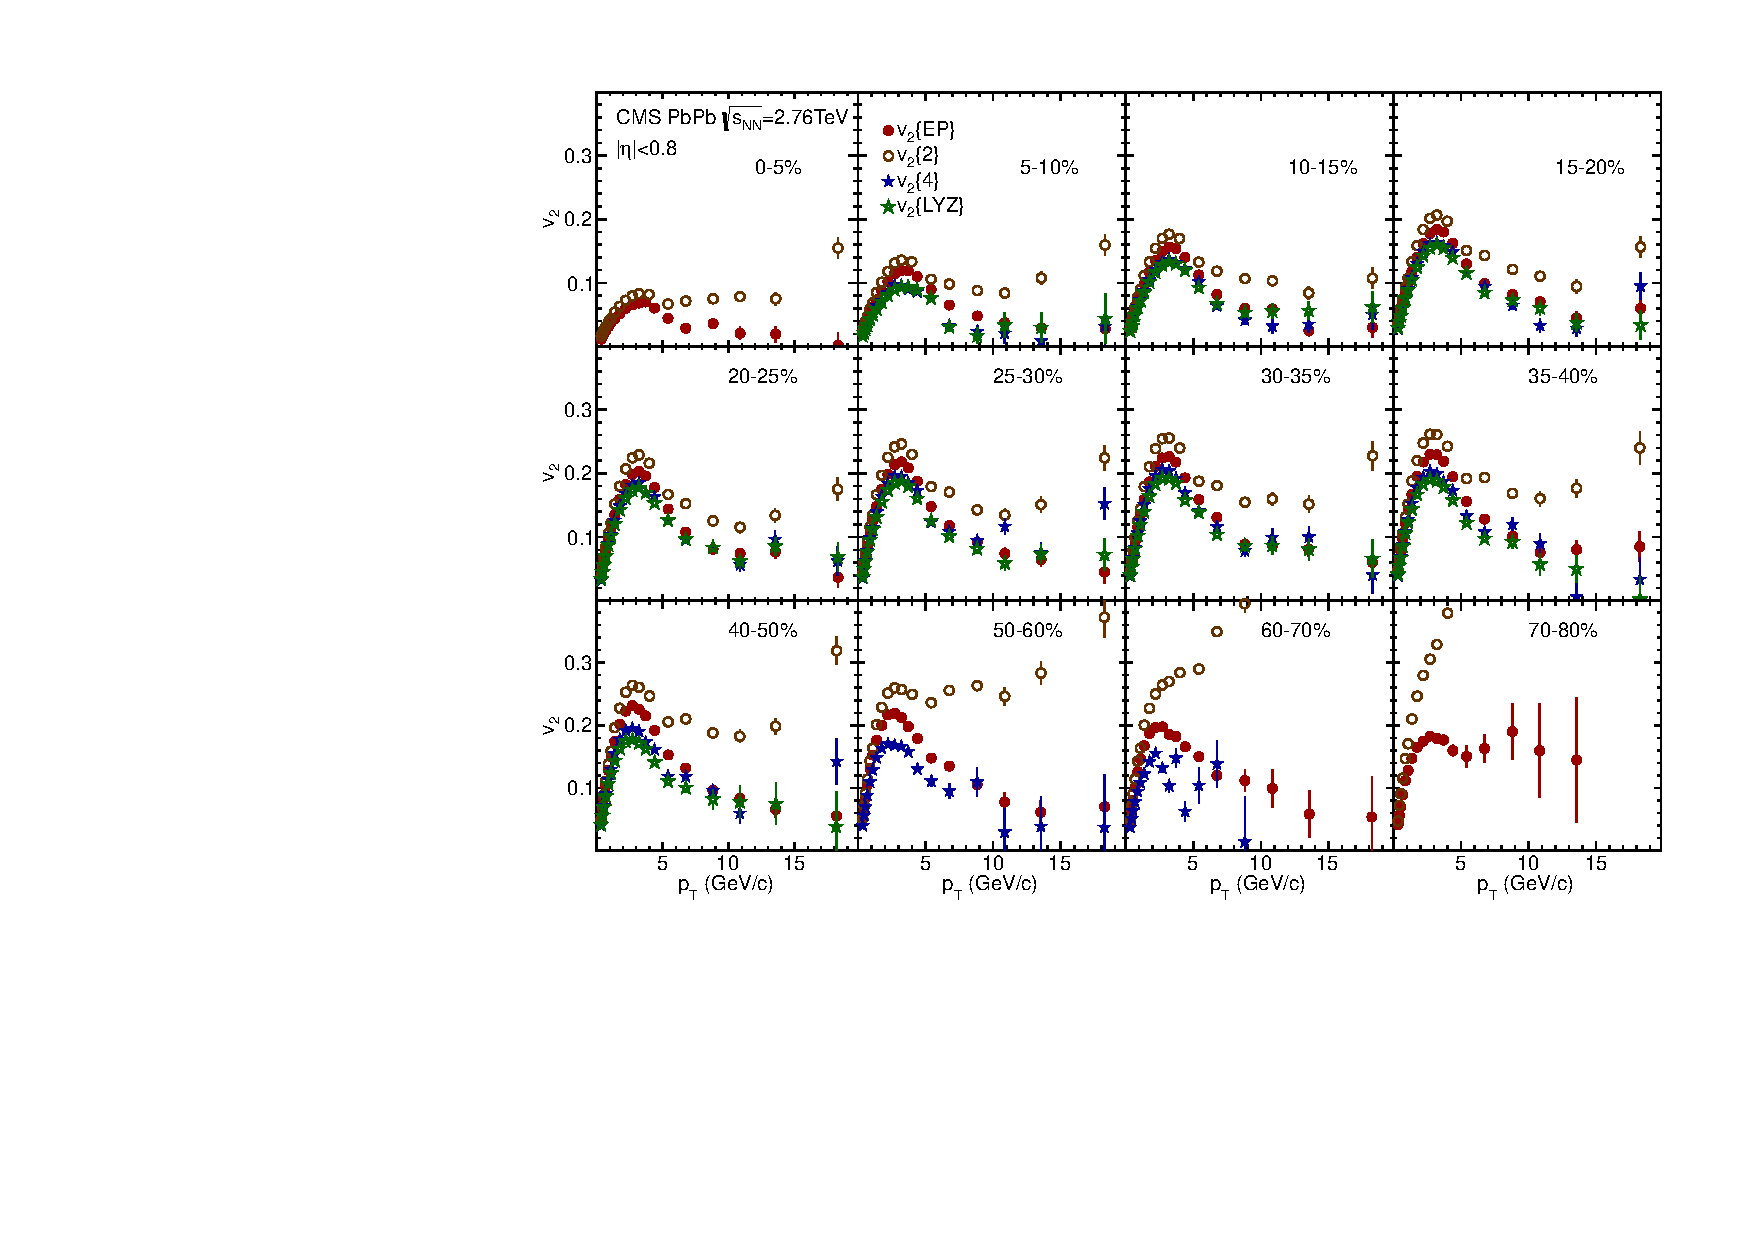
\includegraphics[width=0.98\textwidth]{flowcorrelations_figs/v2_pt_12cen_4methods.pdf}
\caption[]{
CMS data showing $\vtwo(\pT)$ in centrality intervals, using four different methods of extracting
$\vtwo$: event plane (EP), 2-particle cumulants, 4-particle cumulants, and Lee-Yang Zeros.
}
\label{fig:pas:fc:methods}
\end{center}
\end{figure}



